\documentclass{article}
\usepackage[utf8]{inputenc}
\usepackage{graphicx}
\usepackage{float}

\title{Cloud Computing - Notes}
\author{Eduardo Rinaldi - rinaldi.1797800@studenti.uniroma1.it}
\date{June 2022}

\begin{document}
\maketitle
\tableofcontents
\newpage

\section{The big picture of Cloud Computing}
Cloud computing is the product of a set of three main technologies:
\begin{enumerate}
    \item \textbf{Virtualization:} capacity to abstract elements of computing (e.g hardware, storage, etc.). \textit{Hardware virtualization} consists in abstracting hardware resources using software (e.g. vpn or virtual machines). \textit{Software virtualization} or, also known as \textit{application virtualization}, consists in executing an application in an isolated environment (e.g. using \textit{docker}).
    \item \textbf{Web 2.0:} set of technologies that allows to create web applications and not only static/dynamic web pages.
    \item \textbf{Service orientation:} a reference model for cloud computing that base everything on a small building block called "\textit{service}". A service can be seen as a small piece of code that solve a simple task and it can be reused in different kind of applications (e.g. a "login/register" service). So given this, a service should be reusable, programming language and location independent.
\end{enumerate}

\subsection{Business drivers and risks}
Most important cloud computing's business drivers are three:
\begin{enumerate}
    \item \textbf{Capacity planning:} provide the right amount of capacity when needed, acting different strategies: lag strategy (reactive), lead strategy and match strategy (proactive).
    \item \textbf{Cost reduction:} cloud solutions dramatically reduce costs needed to buy and maintain a certain infrastructure. A consumer does not have to worry about maintenance costs (provider responsibility) and also some of the costs are reduced by the fact that most services are payed on-demand (you pay for what you actually use).
    \item \textbf{Agility:} measures the responsiveness to the change, in other words cloud solutions allows to response to an higher/lower demand within few hours.
\end{enumerate}

Even if we have several benefits, this kind of technology brings some risks:
\begin{enumerate}
    \item Increase security vulnerabilities
    \item Limited portability between cloud providers
    \item Reduced governance control
\end{enumerate}

\subsection{NIST definition of cloud computing}

\textit{Cloud computing is a model for enabling ubiquitous,
convenient, \textbf{on-demand network access} to a shared pool of
configurable computing resources (e.g., networks, servers,
storage, applications, and services) that can be rapidly
provisioned and released with minimal management effort or
service provider interaction}

This cloud model is based on \textbf{5 essential characteristics}, \textbf{3 service models} and \textbf{4 deployment models}:
\begin{itemize}
    \item Characteristics:
    \begin{enumerate}
        \item \textbf{On-demand self-service:} relies on orchestration services, programming API, dedicated shell, web interface.
        \item \textbf{Broad network access:} accessible from anywhere and from any device that can connect to internet.
        \item \textbf{Resource pooling:} resources are pooled to serve multiple consumer using a multi-tenant model
        \item \textbf{Rapid elasticity:} is related to \textit{scalability}, is the ability of a system of adapting to workload changes in an automatic manner.
        \item \textbf{Measured services:} user should monitor resources usage so to apply automatic management tasks (e.g. scaling using thresholds, control cost by using alerts, etc.)
    \end{enumerate}
    \item Service models: they help to separate consumer and provider responsibility based on the service type
    \begin{enumerate}
        \item \textbf{Infrastructure as a service (IaaS):} provider is responsible for the infrastructure (i.e. server, storage, virtual machine), everything else is consumer responsibility.
        \item \textbf{Platform as a service (PaaS):} provider is responsibile for the platform (i.e. infrastructure and everything else except for application and data).
        \item \textbf{Software as a service (SaaS):} provider is responsible for every resource given to the consumer, both software and hardware.
    \end{enumerate}
    \item Deployment models:
    \begin{enumerate}
        \item \textbf{Public cloud:} cloud resources are publicly accessible.
        \item \textbf{Private cloud:} cloud resources are private, they act as they are in a virtual private network.
        \item \textbf{Hybrid cloud:} public + private cloud.
        \item \textbf{Community cloud:} cloud infrastructure can be used by consumers of a specific community with a common need.
    \end{enumerate}
\end{itemize}

\subsection{Cloud computing roles}
\begin{itemize}
    \item \textbf{Provider:} for example Amazon AWS, Google Cloud Platform
    \item \textbf{Consumer:} the one who will access to cloud resources (not the application end-user)
    \item \textbf{Auditor:} conduct assessment of cloud services testing performance and security
    \item \textbf{Broker:} third part that helps the negotiation between consumer and provider (helps not in the sector consumers to choose the right services)
    \item \textbf{Carrier:} provide connectivity and transport of cloud services.
    \item \textbf{Resource administrator:} responsible for administrating cloud resources (could be the consumer, the provider or a thirdy part organization)
    \item \textbf{Service owner:} the legal owner of a cloud service (could be the consumer or the provider)
\end{itemize}

\section{Enabling core technologies}
\subsection{Distributed computing}
It's a computing model where computation is broken down into multiple units executed concurrently (i.e. on \textit{multi-node} or \textit{multi-cpu} or \textit{multi-core}), implying different location of computing elements and heterogeneity in terms of hardware and software features. Usually these systems includes:
\begin{itemize}
    \item Framework for distributed programming (e.g. spark)
    \item Inter-process communication (\textbf{IPC}) primitives for control and data
    \item Parallel hardware and networking
\end{itemize}

To give two formal definitions of distributed systems:
\begin{enumerate}
    \item \textit{``A distributed system is a collection of independent computers that
appears to its users as a single coherent system"} [Tanenbaum]
    \item \textit{``A distributed system is one in which components located at networked
    computers communicate and coordinate their actions only by passing
    messages"} [Coulouris]
\end{enumerate}

\subsection{Software architectural styles}
It defines the logical organization of the software components. Two main styles (not the only existing ones) are:
\begin{enumerate}
    \item \textbf{Call and return:} can be based on a classic top-down approach where each component is either a procedure or a subprogram and the calling program pass inputs to procedures which these return an output value when the computation is done; this approach can also follow a layered structure (similar to tcp/ip stack).
    \item \textbf{Independent components:} each component has its own life-cycle and they interact each other. Communication between components is defined by their architecture which can be either ``process based" (on slide ``communicating processes"), i.e. each service is an independent process and each process provides services that can be used by others, or ``event based", i.e. each component publish a list of events which other components can subscribe and define their callback for that event.
\end{enumerate}

One architectural style which is based on independent components is ``\textbf{Microservices}", where basically we have 10s or 100s of small independent services each of which is handled by a small team. These kind of architecture allows us to:
\begin{itemize}
    \item continuously deploy large applications (avoiding to deploy every time the entire application),
    \item easily maintain and scale services, i.e. \textit{x-axis} (\textbf{cloning}), \textit{y-axis} (\textbf{functional decomposition}), \textit{z-axis} (\textbf{data partitioning})  scaling,
    \item test new technologies; each service is independent, this also means that they're vendor independent,
    \item isolate faults.
\end{itemize}
Drawbacks of microservices are given by the amount of complexity they introduce (e.g. decompose a system into services, development and testing).
\subsection{System architectural styles}
It defines the physical organization of processes and components over a distributed system. Two styles:
\begin{enumerate}
    \item \textbf{Client-server:} composed by three main components which are: presentation, logic and data storage. Based on how these three components are arranged we can have \textit{thin-client} (i.e. logic is performed on server) and \textit{fat-client} (i.e. logic is performed on client). A distributed approach is given by multi-tier model which consists in making components conceptual layers called tiers. (classic model is a 2-tier approach, because we only have one client and one server)
    \item \textbf{Peer-to-Peer:} each component (peer) can be both client and server at the same type, consistency here is maintained by consensus algorithms (like paxos or the ones used in blockchain)
\end{enumerate}
\subsection{IPC models}
Communication between processes in distributed systems can be achieved by different IPC models:
\begin{itemize}
    \item \textbf{Remote Procedure Call (RPC):} use a client/server approach, where the client call for the remote procedure and the server process and return the procedure result. The RPC infrastructure is responsible for marshaling/un-marshaling and for handling requests between client and server. Developers should only worry about defining and registering the remote procedure on the server and define the client code that invokes the remote procedures.
    \item \textbf{Distributed objects:} very similar to RPC but for object oriented paradigm (stateful approach).
    \item \textbf{Service Oriented Architecture (SOA):} a service encapsulate a software component where boundaries are explicit (simple interfaces), service is autonomous, services share schemas and contracts (those defines the structure of the messages that can be sent or received) and their compatibility is defined by policies. With this approach services can be both consumer and provider and they can belong to different domains or organizations. Services are then managed in two ways:
    \begin{enumerate}
        \item \textbf{Orchestration:} there's an entity which manage the communication between services
        \item \textbf{Choreography:} there's no central entity which manage communication (this avoid single point of failure), but instead services communicates each other directly.
    \end{enumerate}
\end{itemize}

\begin{figure}[H]
    \centering
    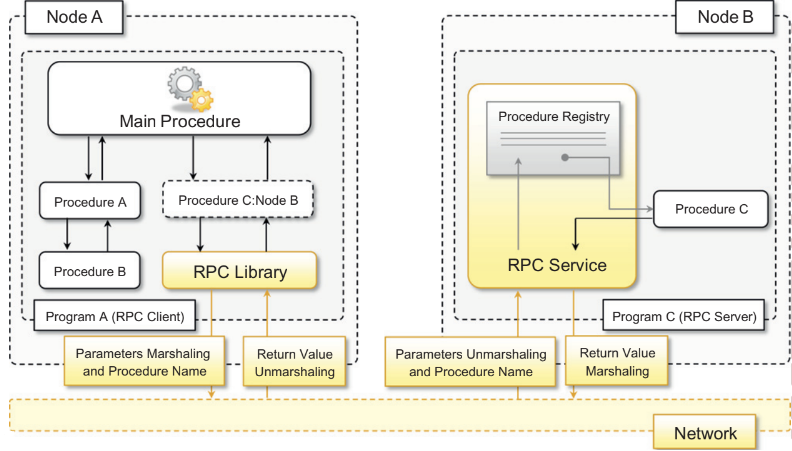
\includegraphics[width=3.5in]{imgs/rpc.PNG}
    \caption{RPC}
    \label{fig:rpc}
\end{figure}
\begin{figure}[H]
    \centering
    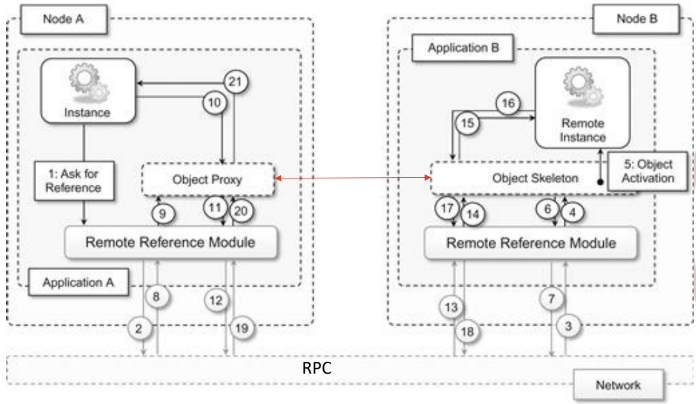
\includegraphics[width=3.5in]{imgs/distributedobjects.PNG}
    \caption{Distributed objects}
    \label{fig:rpc}
\end{figure}
\begin{figure}[H]
    \centering
    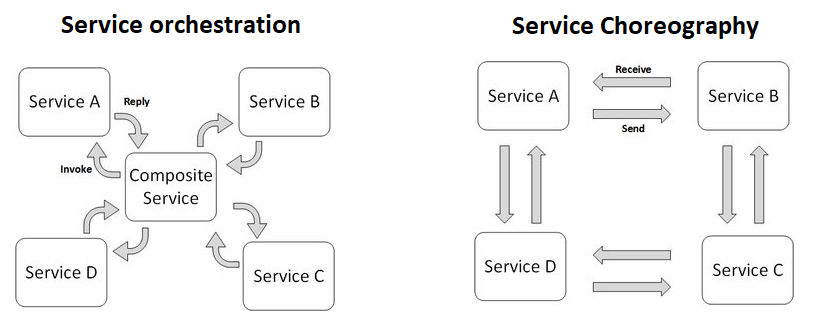
\includegraphics[width=3.5in]{imgs/orchestration vs choreography.PNG}
    \caption{SOA service managing}
    \label{fig:rpc}
\end{figure}

\subsection{Differences between SOA and Micro-services}
Even if at a high level they seems to be the same things we can spot some differences in:
\begin{itemize}
    \item \textbf{Communication mechanism:} SOA uses an Enterprise Service Bus as a communication middle-ware, creating a single point of failure, providing a slow communication with an high configuration and maintenance complexity. Micro-services instead use lightweight and open-source technologies like REST.
    \item \textbf{Data:} SOA usually have shared database, while each micro-service has its own database.
    \item \textbf{Services' size:} usually SOA is used for integrating monolithic applications, so that they can communicate each other, micro-services instead are very small pieces of software (a single application could easily be composed by hundreds of services).
\end{itemize}

\section{Virtualization}
Virtualization is a technique that by using software simulates hardware in order to create a virtual system. This technique has been widely explored since it allows us to better deal with: unused hardware and software resources, lack of spaces, administrative costs (similar to cloud computing's drivers).
In addition to these, we can say that virtualization:
\begin{itemize}
    \item \textbf{Increase security:} provides an isolation layer between guest os and host os (in terms of operations and data).
    \item \textbf{Execution is managed:} allows for an array of possible computing scenarios (i.e. guest programs and environments can be shared, aggregated, emulated or isolated).
    \item \textbf{Portability:} a virtual machine image can be easily duplicated and instantiated on another host machine. (e.g. java code can be executed on any os running a jvm).
\end{itemize}

\textbf{Virtualization techniques} can be split in to two macro-categories: \textit{Hardware} (or \textit{System}) \textit{level virtualization} and \textit{Software level virtualization}.

\begin{figure}[H]
    \centering
    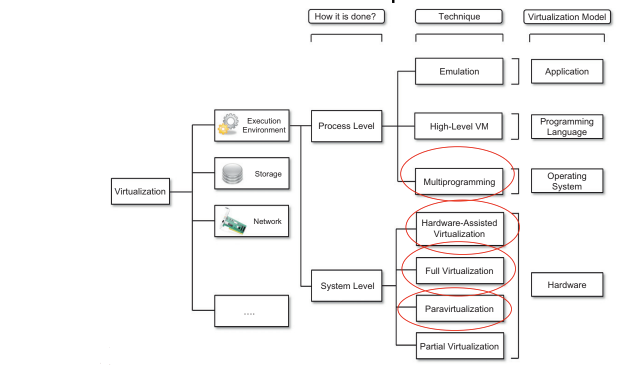
\includegraphics[width=4in]{imgs/virttech.PNG}
    \caption{Virtualization techniques}
    \label{fig:virttech}
\end{figure}

\subsection{Hardware / System level virtualization}
This kind of a approach consists in using an \textbf{Hypervisor} (a.k.a. \textbf{Virtual Machine Manager - VMM}) so to emulate and manage CPU status on guest OS. An Hypervisor is a further abstraction layer that runs in supervisor mode (i.e. privileged mode) and it's placed between a virtual machine instance and, the operating system (\textit{type II}) or directly the hardware (\textit{type I}). Generally, an hypervisor is composed by:
\begin{itemize}
    \item \textbf{Dispatcher:} entry point which dispatch instructions to either allocator or the interpreter
    \item \textbf{Allocator:} manage system resources available to VM. If an instruction change VM's current resource allocation, the allocator will be invoked.
    \item \textbf{Interpreter:} every time the virtual machine want to execute a privileged instruction a trap is triggered and the corresponding routine is executed.
\end{itemize}
An hypervisor, to be defined as so, should respect 3 properties:
\begin{enumerate}
    \item \textbf{Equivalence:} guest should behave like if it's running on physical host.
    \item \textbf{Resource control:} complete control over virtualized resources.
    \item \textbf{Efficiency:} a good fraction of instructions should be executed without the intervention of VMM.
\end{enumerate}

\subsubsection{Full virtualization}
This approach consists in scanning the instruction streams and, non-privileged instruction are directly run on hardware, while privileged instructions are trapped and VMM tries to emulate their behavior by using \textbf{binary translation}.

Binary translation is an emulation technique where instructions of source instruction set are converted into a target instruction set; this conversion can happen:
\begin{itemize}
    \item Statically: all code in an executable file is converted without running the code
    \item Dynamically: code is converted at run-time, usually by looking at short sequence of instructions. This introduce a run-time overhead that is reduced by caching mechanism.
\end{itemize}

\subsubsection{Hardware assisted virtualization}
A \textbf{set of additional instructions is added}, in order to control the start/stop of a VM, allocate memory pages, maintain CPU state for VMs. Example of HW-Assisted virtualization are \textit{Intel-VT} and \textit{AMD-V}.

\subsubsection{Para-virtualization}
It's a technique that presents a software interface to the virtual machines, similar (not identical) to the underlying hardware-software interface. The intent is to reduce the execution time required by those instructions which would run faster into a non-virtualized environment. Para-virtualization requires substantial modifications to guest OS.

\subsection{Virtual machine migration}
VM should be portable, that means that they should be moved from an host to another without too much difficult. For achieving this we have two types of migrations:
\begin{itemize}
    \item \textbf{Offline:} vm is stopped, moved and restarted.
    \item \textbf{Live:} vm is transferred as it is not stopped while migrations is happening (without generating a service discontinuity).
\end{itemize}

Live migration consists in the following steps:
\begin{enumerate}
    \item Start migration: VM and the destination host are determined (can be done either by human or by automatic strategies such as load balancing)
    \item Transfer memory: send VM memory to destination node (this ensure service continuity) in rounds. In first round all memory is copied and then until dirty portion of memory is small enough to handle final copy, it recopies data changed w.r.t. last round.
    \item Suspend VM: send CPU and network states and suspend the source VM.
    \item Activate destination host: reload states and recover execution of programs, then redirect network connection to the new VM. Old VM is removed from source host.
\end{enumerate}

\subsection{Software level virtualization}
This kind of virtualization, also called \textbf{containerization}, can be seen as an evolution of \textit{chroot} mechanism, it leverages on multi-programming techniques at OS level, thus implying no VMM and no HW emulation is required, instead the result consists in multiple VMs sharing same host operating system. Fundamentals for containerization are: \textbf{namespaces}, \textbf{CGroups} and \textbf{UnionFS}.

\subsubsection{Namespace}
A namespace wraps global resource (e.g. CGroups, IPC, Network, Mount, PID, etc.) in an abstraction so that processes within a namespace perceive that they have their own instance of it. Changes to a global resource are visible only to processes that are member of the namespace.
\subsubsection{CGroups}
It's a Linux kernel feature that allows processes to be organized in hierarchical groups whose usage of resources can be monitored and/or limited. The kernel's cgroup interface is provided through pseudo-filesystem called cgroupfs.
\subsubsection{UnionFS}
Allows administrator to keep files physically separated but logically unified into a single view. Each physical filesystem or directory is called ``\textit{branch}", while the UnionFS result is called ``\textit{merge}". 

To each branch is assigned a priority and a branch with higher priority overrides branches with lower one. 

This filesystem operates on directories, so if a directory exits in two branches then the content of the union directory is the combination of these two. It also automatically removes any duplicated directory entry by keeping only the file content and attributes of the higher priority branch.

\subsection{Docker}
Docker is a set of PaaS products that use OS-Level virtualization and containers run directly within the host machine's kernel. On the latter is installed the \textbf{Docker Engine}, which is an application that provides CLI interfaces to interact with the server (called \textbf{Docker daemon}).

\begin{figure}[H]
    \centering
    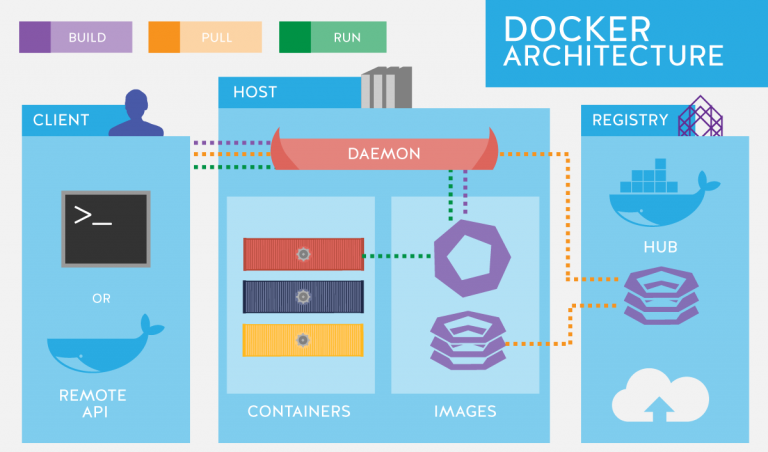
\includegraphics[width=4in]{imgs/dockerarchitecture.png}
    \caption{Docker architecture}
    \label{fig:dockerarchitecture}
\end{figure}

\subsubsection{Storage options}
\begin{figure}[H]
    \centering
    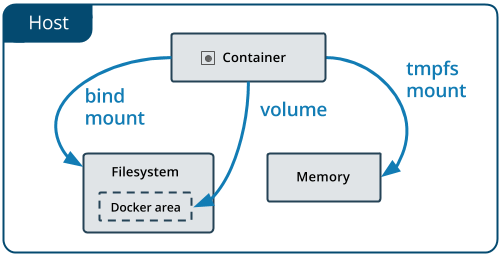
\includegraphics[width=4in]{imgs/types-of-mounts.png}
    \caption{Type of mounts}
    \label{fig:typeofmounts}
\end{figure}
\begin{itemize}
    \item \textbf{Container writable layer:} all files created inside a container are stored in it. Data does not persist when container no longer exists and it can be difficult to share data with other containers.
    \item \textbf{Volume:} created and managed by docker (isolated from the host) is stored within a directory on the docker host.
    \item \textbf{Bind mount:} a file or directory on host machine is mounted into a container. Dependence on the filesystem makes this system non-portable, but faster than volumes.
    \item \textbf{tmpfs:} a memory area outside the container writable layer, which is shared with host or is in the container namespace. It's temporary and only persisted in the host memory. Available only on Linux hosts and not sharable among containers.
\end{itemize}
\subsubsection{Network options}
With docker is possible to connect container each other or connect container to non-Docker workloads by using the following network drivers:
\begin{itemize}
    \item \textbf{bridge:} default network driver, used when applications run in standalone containers that need to communicate.
    \item \textbf{host:} remove network isolation between container and host and uses host's networking directly (for standalone containers).
    \item \textbf{overlay:} connect multiple docker daemons together, allowing communication between containers or services on different daemons.
    \item \textbf{macvlan:} allows to assign a MAC address to a container, making it appear as a physical device in the network.
    \item \textbf{none:} disable all networking.
\end{itemize}

\section{Automatic Computing}
\textbf{Data-centers} are large scale complex systems containing thousands of servers spread around the world. These structures comes with several challenges that cannot be performed only by humans, ranging from \textbf{handling HW/SW} (e.g. failures, updates, other operations) for guaranteeing \textbf{Service Level Agreements} (SLA). \textbf{Autonomic Computing} is a solution to this problem: field humans only if needed by making the system capable to manage itself.

\subsection{Autonomic Computing}
Given an high-level objective from system administrator, autonomic computing systems can manage themselves by performing a \textbf{MAPE} cycle of actions:
\begin{itemize}
    \item \textbf{Monitor:} check system state (e.g. retrieve cpu load)
    \item \textbf{Analyze:} perform some analytic on monitored data (e.g. aggregation, prediction, comparison) 
    \item \textbf{Plan:} decide which action should be taken for keeping the system in the desired state
    \item \textbf{Execute:} execute the planned action
\end{itemize}
Autonomic computing systems have the following properties:
\begin{itemize}
    \item \textbf{self-configuration:} ability to configure and reconfigure itself under various circumstances (e.g. perform software installation and updates).
    \item \textbf{self-healing:} ability to recover from failures (e.g. deal with os crashes).
    \item \textbf{self-protection:} ability to detect and mitigate attacks (e.g. prevent attack, deal with a successful attack).
    \item \textbf{self-optimization:} ability to constantly monitor for optimal solution (e.g. auto-scaling).
\end{itemize}

\subsection{Auto-scaling}
\textbf{Scalability} measures the trend of performance with an increasing workload and a system is \textbf{scalable} if under that increasing workload it can maintain its performance by allocating new resources. Scaling mechanisms can be performed by:
\begin{itemize}
    \item Replication of application (usually done on monolithic applications)
    \item Replication of an application components (usually done on micro-services applications)
\end{itemize}
Auto-scaling mechanisms usually define 3 things: \textit{scaling condition} (e.g. an event triggered by a threshold exceeded), \textit{scaling action} (e.g. scale in/out, scale up/down), \textit{scaling amount} (e.g. add 3 VMs).

\subsubsection{Auto-scaling conditions}
Auto-scaling algorithms can be:
\begin{itemize}
    \item \textbf{Reactive:} take action \textit{while} the performance are decreasing. This kind of algorithms can be based on thresholds (heuristic based, so no optimal solution) or combination of them, or either based on a mathematical model of the system which provides the scaling action that should be performed (could provide optimal solution).
    \item \textbf{Proactive:} predict performance metrics and takes decision few minutes ahead.
\end{itemize}
and they can be based on either a ``\textbf{simple scaling}" approach or a ``\textbf{step scaling}" one. The difference stands in the fact that in simple scaling we have a \textit{cool down} time just after the scaling action has been performed, while in the other one there's no cool down. This results in lower reactivity in simple scaling and in a ``\textit{ping-pong}" problem in step scaling (e.g. increasing the number of VMs and then immediately decreasing them, and so on).

\bigskip
Instances that are just being started and still cannot perform at their maximum potential are considered in ``\textit{warm-up}" state.
At a given time $t$, the ``performance metric value" used by the scaling condition is calculated by taking the average of the performance metric value of all the instances that are \textbf{not in warm-up state}.
$$V_t = \frac{1}{N_t}\sum^{N_t}_{i=1}{PM(VM_i)}$$

\begin{figure}[H]
    \centering
    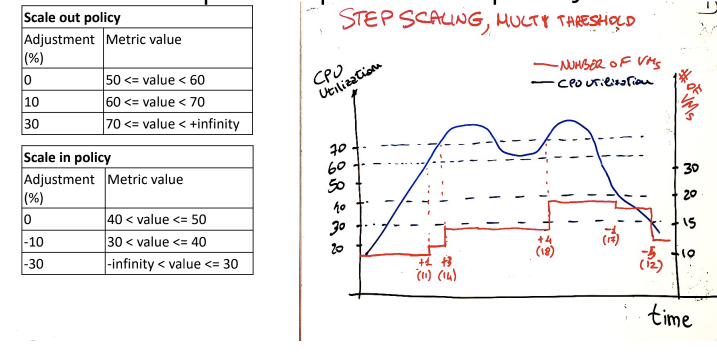
\includegraphics[width=4in]{imgs/exampleofscaling1.PNG}
    \caption{Example of scaling}
    \label{fig:eos1}
\end{figure}

\begin{figure}[H]
    \centering
    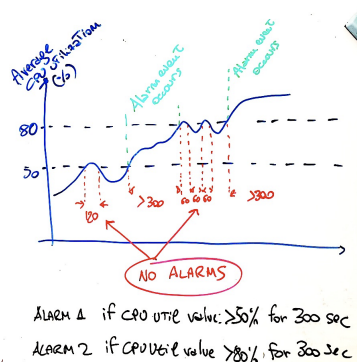
\includegraphics[width=3in]{imgs/exampleofscaling2.PNG}
    \caption{Example of scaling}
    \label{fig:eos2}
\end{figure}

\subsubsection{Auto-scaling amount}
Also called scaling policy, it defines the amount of instances that should be up. It can be defined in 3 ways:
\begin{itemize}
    \item \textbf{Change in capacity:} define the number of instances \textit{to add}.
    \item \textbf{Exact capacity:} define the number of instances that should be up after the scaling.
    \item \textbf{Percentage:} like the first one, but defined using percentages over the actual number of instances.
\end{itemize}

\subsection{Auto-scaling in AWS}
The idea is to define 3 things:
\begin{enumerate}
    \item \textbf{Auto-scaling group:} group of EC2 instances that shares similar characteristics.
    \item \textbf{Launch configuration:} EC2 template used by Auto-scaling group for new EC2 instances.
    \item \textbf{Scaling policy:} policy that determine scaling action
\end{enumerate}
Scaling plan and launch configurations are associated to a group, which for the latter can be defined several scaling policies (at least one must be defined).

\subsection{Orchestration with Ansible}
Data-centers have specialized platforms for automating tasks like provisioning, configuration, patching and/or monitoring. An example of these platforms is \textbf{Ansible}, a state-less orchestration tool which does not require to install any software on the remote machine (i.e. \textbf{agent-less}), not bringing any kind of overhead when management is not running. It runs following a ``\textit{push model}", it means that control instructions (management instructions) are sent to remote machines through existing technologies like \textit{SSH} on Linux, or \textit{WinRM} on Windows. Fundamentals components of Ansible are:
\begin{itemize}
    \item \textbf{Host inventory:} set of hosts on which are applied automation tasks
    \item \textbf{Playbook:} a series of ``plays", each of which is a set of tasks that can target one, many or all the hosts in the inventory. A playbook is defined through a \texttt{.yaml} file and it comes with a variety of features that allows to express conditional execution of tasks, gather system variables from remote machines.
    \item \textbf{Module:} a task to be performed, in practice a small piece of code for doing a specific task. Each module is run only if needed, and this needing condition can be expressed by using preconditions.
\end{itemize}

\subsection{Kubernetes}
Also referred to as K8s is a platform for managing containerized workloads and services, so it basically does the following:
\begin{itemize}
    \item Service discovery (find services actually running) and load balancing.
    \item Automatically mount storage (storage orchestration).
    \item Automatically bring container into, so called, ``desired" state.
    \item Distributes containers between nodes so as to have the best use of resources
    \item Restarts, kill, replace and does not advertise faulty containers
    \item Secret and configuration management (e.g. secret keys, env variables)
\end{itemize}

A K8s cluster can be split in to two macro entities category: \textbf{control plane} and \textbf{k8s nodes}. 
\begin{figure}[H]
    \centering
    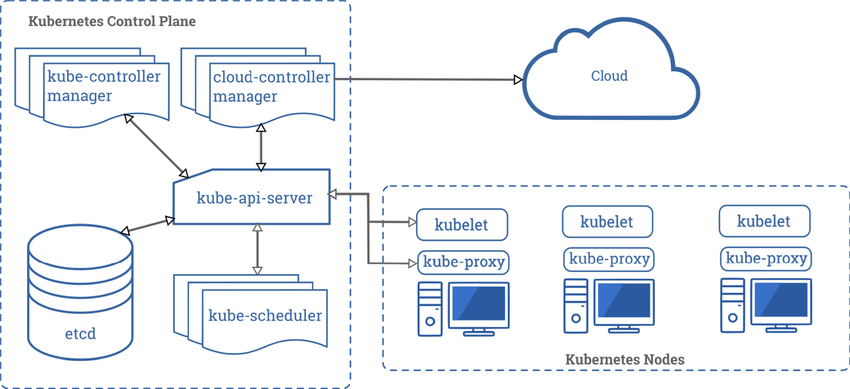
\includegraphics[width=4in]{imgs/The-control-components-of-K8S-45.png}
    \caption{Kubernetes cluster components}
    \label{fig:k8scomp}
\end{figure}

Kubernetes is also based on three main types of objects:
\begin{itemize}
    \item \textbf{K8s objects:} persistent entities used by k8s for representing the state of the cluster (e.g. which containerized apps are running and on which nodes, resource available, policies, and so on)
    \item \textbf{K8s pods:} smallest deployable units of computing that can be created and managed in k8s. It's a group of one or more containers with shared storage and network resources. The shared context is a set of Linux namespaces.
    \item \textbf{Node condition} (e.g. condition type, status, reason, ..).
\end{itemize}

\subsubsection{K8s Nodes}
Nodes are virtual or physical machines on which to run containerized workloads, they are member of a k8s cluster and are managed by the control plane. Nodes can either manually register or self-register themselves to control plane (API-Server).

Once a node is created the control plane checks for its validity and returns the node status containing information like: address, capacity and node condition (e.g. condition type, status, reason, ..).

A node is generally composed by 3 components:
\begin{enumerate}
    \item \textbf{kubelet:} controls that container described in PodSpec are running in a pod and their status is healthy.
    \item \textbf{kube-proxy:} allow communication to cluster's pods from outside or inside the cluster
    \item \textbf{Container run-time:} container engine (e.g. docker)
\end{enumerate}

\subsubsection{Control plane components}
Control plane usually runs on a dedicated server or VM and it includes the following components:
\begin{itemize}
    \item \textbf{kube-api-server:} front-end of the k8s control plane which can be horizontally scaled.
    \item \textbf{etcd:} key-value store used for storing all cluster data.
    \item \textbf{kube-scheduler:} watches for new pods with no assigned node, and selects best node for them to run on, according to their requirements for resources. So basically the scheduler first finds feasible nodes for a pod (filtering process) and then runs a scoring phase for choosing the best node among feasible nodes. It's possible to implement a custom scheduler.
    \item \textbf{kube-controller-manager:} runs controller processes such as node controller, job controller, ...
    \item \textbf{cloud-control-manager:} link k8s cluster with a specific cloud provider's API
\end{itemize}

\section{Cloud data storage}
Multiple forms of data storage are used in cloud systems (e.g. distributed file systems or databases), the common goals are: massive \textbf{scaling} on demand, high \textbf{availability} and \textbf{simplified developing} and \textbf{deploying} methodologies. For achieving this several things are needed to take into account.

\subsection{Atomicity}
It's the property which guarantee that multi-step operations are executed as if they were single-step operations (i.e. without any interruption). Atomicity needs HW support which must provide two basic primitives operations: \textbf{test-and-set} and \textbf{compare-and-swap}. These two allows us to implement critical section handling mechanisms like \textit{semaphores}, \textit{lock} or \textit{monitors}.

\bigskip
Two kinds of atomicity:
\begin{itemize}
    \item \textbf{All or nothing:} two phases, the pre-commit phase which consists in a set of operations that are either all finish or none at all (strategy for masking failures during execution).
    \item \textbf{Before or after:} result of every read or write is the same as if that read or write occurred either before or after any other read or write (necessary for coordination of concurrent activities).
\end{itemize}

\subsection{Storage models}
Storage model describe the layout of the data structure of the physical model (disk or solid state) and is desirable to have read/write coherence, before-or-after and all-or-nothing atomicity. Two models:
\begin{itemize}
    \item \textbf{Cell storage model:} assumes that storage consists of fixed size cells and that each object fits exactly one cell. Read/write coherence is not guaranteed.
    \item \textbf{Journal storage model:} stores records consisting of multiple field and it keep tracks of all the versions of all the variables stored (log). It consists of two components: the \textbf{manager} and the \textbf{cell storage}. The user does not directly access to the storage, but instead it can request to the manager to: create a new action, read/write a cell or commit/abort an action. An online transaction is basically an all-or-nothing action which record the action into the journal storage and then apply the change in the cell storage overwriting the previous version.
\end{itemize}

\subsection{Google file system}
GFS has been designed after a careful analysis of the file characteristics and of the access models:
\begin{itemize}
    \item File size ranging from few GB to 100s of TB. GFS uses thousands of inexpensive components to provide petabyte of storage.
    \item Files are often \textit{read sequentially} and random writes operation are rare compared to appending operations (this allow them to use HDDs over expensive SSDs).
    \item Response time is not a main requirement, data are processed in bulk.
    \item High reliability to hw/sw failures or human errors.
    \item Relaxed consistency model to simplify the system implementation.
\end{itemize}

GFS architecture is accessed by multiple clients and consists of a single \textbf{master} and multiple \textbf{chunk-servers}. Files are stored in chunk-servers as Linux files and are organized in chunks of fixed size (64 MB). This choice gives improvements over performances such as: reduced time-to-search for a specific file, increase likelihood of locality principle, optimize performances for large files. For reliability, each chunk is replicated on 3 chunk-servers.

\bigskip
The master maintain file system metadata such as the namespace, access control information, mapping from files to chunks, current location of chunks. Having a single master simplify the system design, but its involvement should be minimized in order to avoid SPOF or bottlenecks. Master handle file creation, but instead it does not handle any kind of read/write operation (i.e. clients never r/w data through master). Information regarding where each chunk replica is actually stored is retrieved during start-up phase or whenever a new chunk-server join the cluster.

\bigskip
Clients do not cache file retrieved by chunk-servers (because of their big size), but instead they cache metadata provided by the master when they ask for a specific file (they ask for chunk location).

\bigskip
In case of failure, master recovers its file system state by replaying the operation log (supported by checkpoints for speeding up this process).

\subsection{Hadoop filesystem (HDFS)}
Hadoop provides a distributed filesystem and a framework for analysis and transformation of big dataset using \textit{MapReduce paradigm}. HDFS is based on a Master/Slave model, in which the master (called \textbf{NameNode}) stores metadata, and application data are stored in slaves servers called \textbf{DataNodes}. File content is split into large blocks of fixed size (64-128 MB) which are replicated on multiple DataNodes for reliability (similar concept to chunk in GFS).

\subsection{NoSQL datastore}
Cloud applications are often based on ``\textit{online transaction processing}" (\textbf{OLTP}), which usually requires low response time. This could be achieved in two ways: \textit{(1)} by using a caching system and/or \textit{(2)} by scaling those applications. Scalability (horizontal scalability) in OLTP is a big problem since issues of consistency among distributed copies can surely happen, especially by using a relational database; that because those kind of db \textit{must} preserve \textbf{ACID properties}.

\bigskip
Non-relational database models (\textbf{NoSQL}) allows us to relax on the consistency property, allowing data to be inconsistent and by introducing the concept of ``\textbf{eventual consistency}" which means that data at some future point in time will be consistent, instead of enforcing it when data is ``committed" (something like a lazy approach).

\subsubsection{Google Big Table}
It's a storage system designed and developed by Google which provides high scalability, availability and performance and it's meant to be used in \textit{throughput-oriented}, \textit{batch-processing} and \textit{latency-sensitive} jobs.

Big table is a sorted map which corresponds to the following mapping function:
$$ f : string \times string \times timestamp \rightarrow string $$

or in another way: 

\bigskip 
(row: \texttt{string}, column: \texttt{string}, time: \texttt{int64}) $\rightarrow$ \texttt{string}.

\paragraph{Big table row} is an arbitrary string of maximum 64KB, but usually it ranges from 10 to 100 bytes. Read and write operations are atomic and rows are partitioned into \textbf{tablets}, the unit base for load balancing. Keep in mind that reading small ranges is very efficient, so users should exploit this for improving locality. 

\paragraph{Big table column} grouped into sets called \textbf{column families}. A column key structure is typically \textit{family:qualifier}, and data stored in the same family are of the same type.

\paragraph{Big table timestamp} allows to version control cell's data. Versions are indexed by timestamp, which are sorted in decreasing temporary order so that the most recent version is the first to be read. The assignment can be performed by either the big table itself, or by the client application (collision handling required). Versions are garbage collected by only keeping last n versions of a cell and by keeping only new-enough versions (e.g. latest 7 days).

\bigskip
Big table architecture is based on GFS so it's a master/slave architecture in which a BigTable cluster can store multiple tables and each table is composed by several tablets. The architecture:
\begin{itemize}
    \item \textbf{Master} is responsible for assigning tablets to tablet servers, detect add/delete of tablet servers in the cluster, balancing tablet-server load and handle schema changes.
    \item \textbf{Tablet servers} can be dynamically added or removed to accommodate the workload and each tablet server is responsible to manage a set of tablets, handle read and write requests, split tablets that has grown too much
\end{itemize}

Two other building blocks of this system are:
\begin{enumerate}
    \item \textbf{SSTable:} file format used to store BigTable data. Contains sequence of blocks and corresponding block index.
    \item \textbf{Chubby:} provides distributed lock mechanisms based on files and directories. It's used for ensuring that there's at most one master active, store bootstrap location of BigTable data, discover tablet server and finalize their death, store BigTable schema information, store access control lists.
\end{enumerate}

\subsubsection{Amazon's DynamoDB}
Highly available, scalable and distributed key-value store model, used for managing state of services which require very high reliability. It's based on optimistic replication techniques (i.e. replicas can diverge but at some point in time they will be consistent), which are used for increasing the availability and decreasing latency. Changes are allowed to propagate to replicas but conflicts must be detected and resolved, usually using a consensus algorithm. A smart way of resolving conflicts (used by DynamoDB) is to always allow writes and then conflicts are resolved at read time, so only when needed.

\paragraph{Key design principles} incremental scalability, symmetry, decentralization, heterogeneity.
\paragraph{System interface} consists of two main functionalities:
\begin{enumerate}
    \item \texttt{Get(key)}: locate object replicas associated with the key, returning a single object or a list of versions of it.
    \item \texttt{Put(key, context, object)}: locate where the object should be placed based on the associated key.
\end{enumerate}

\paragraph{Partitioning algorithm} we can see the cluster as an hash table in which each node is a bucket. Given a key, to determine item location, the item's key is hashed to yield it's position. The uniform distribution is given by a good hash function. Virtual nodes concept is introduced for nodes that become unavailable: load handled by this node is distributed across all other nodes until a new node join the system.

\paragraph{Replication} for achieving high availability data is replicated on multiple nodes, let's say $N$ hosts. Data is then replicated to N-1 clockwise successor nodes in the ring. The ring is given by assigning a range of hash values to each node.
\end{document}
